\section{UML class diagrams characteristics} % (fold)
\label{sec:uml_class_diagrams_characteristics}
\begin{figure}
  \begin{center}
    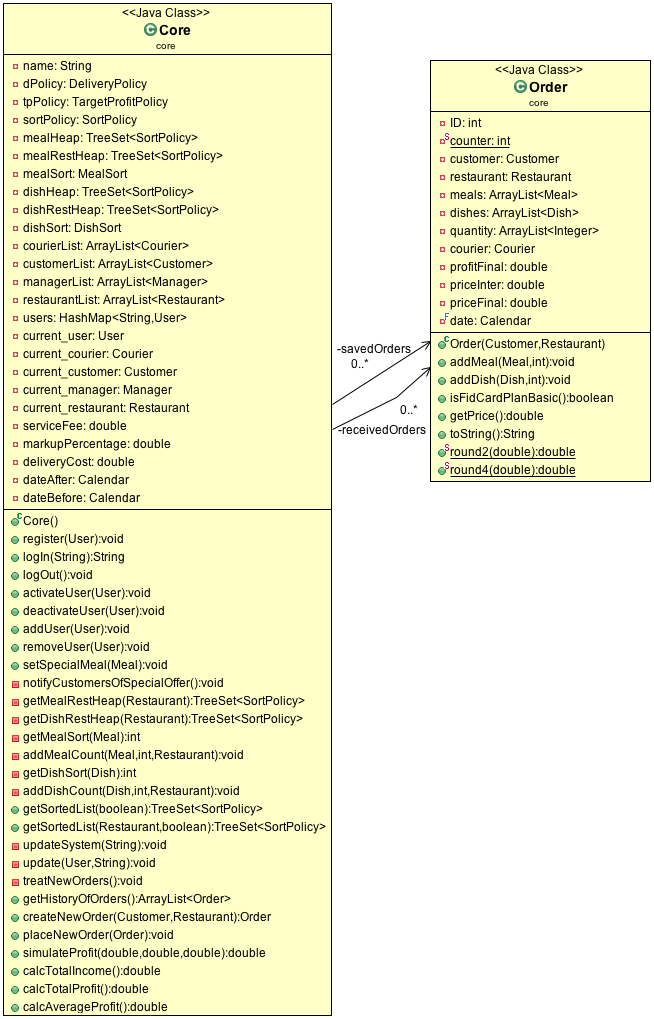
\includegraphics[scale=0.57]{./img/CoreDiagram.png}
    \end{center}
  \caption{\umld \Core~and \Order.}
  \label{fig:core_order_uml}
\end{figure}
\begin{figure}
  \begin{center}
    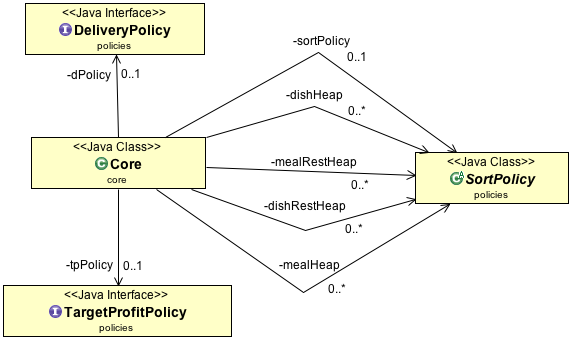
\includegraphics[scale=0.5]{./img/CoreToPolicies.png}
    \end{center}
  \caption{\umld \Core~and its policies objects.}
  \label{fig:core_policies_uml}
\end{figure}
\begin{figure}
  \begin{center}
    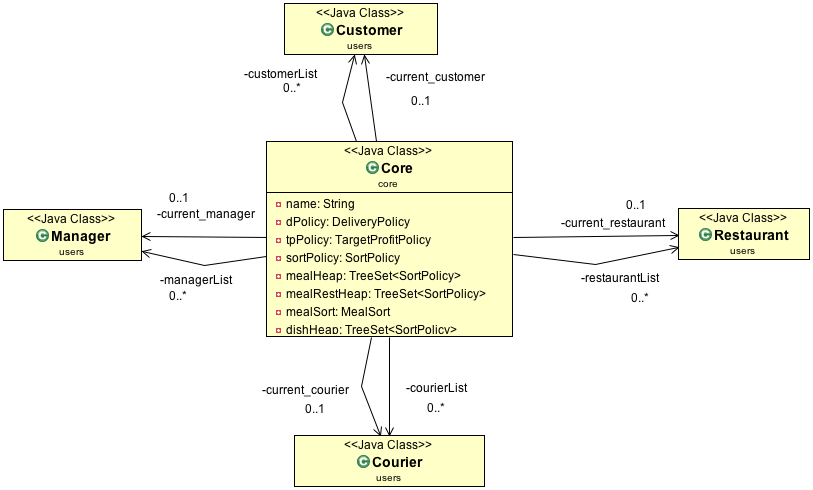
\includegraphics[scale=0.5]{./img/CoreToUsers.png}
    \end{center}
  \caption{\umld \Core~and its link to users.}
  \label{fig:core_users_uml}
\end{figure}
\begin{figure}
  \begin{center}
    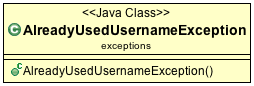
\includegraphics[scale=0.57]{./img/Exceptions.png}
    \end{center}
  \caption{\umld Exception.}
  \label{fig:exception_uml}
\end{figure}
\begin{figure}
  \begin{center}
    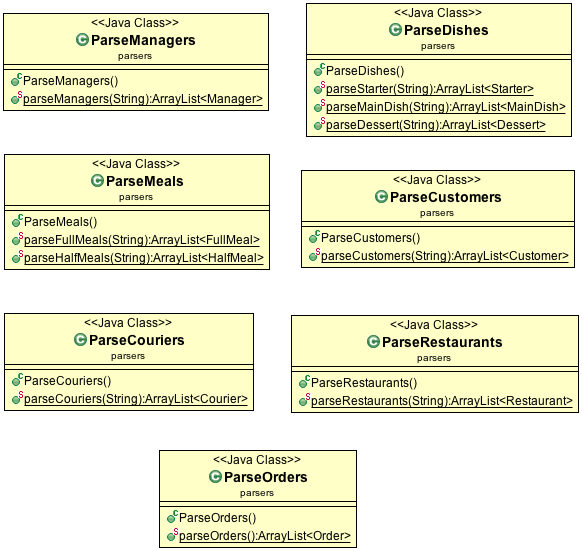
\includegraphics[scale=0.5]{./img/Parsers.png}
    \end{center}
  \caption{\umld Parsers.}
  \label{fig:parsers_uml}
\end{figure}
\begin{figure}
  \begin{center}
    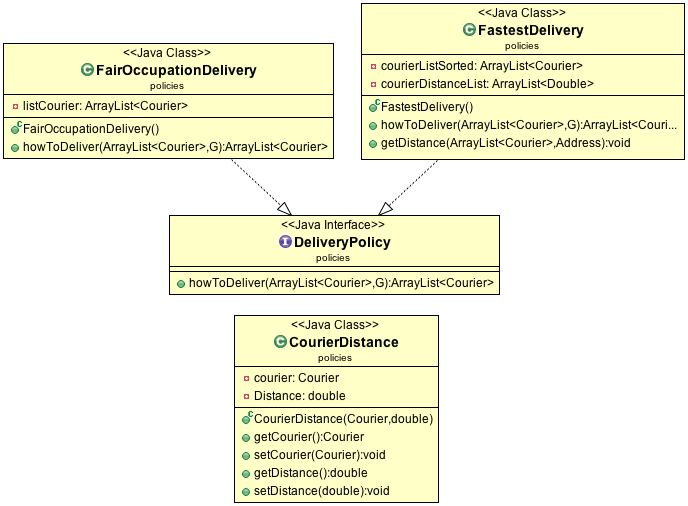
\includegraphics[scale=0.5]{./img/DeliveryPolicy.png}
    \end{center}
  \caption{\umld Delivery policy.}
  \label{fig:delivery_uml}
\end{figure}
\begin{figure}
  \begin{center}
    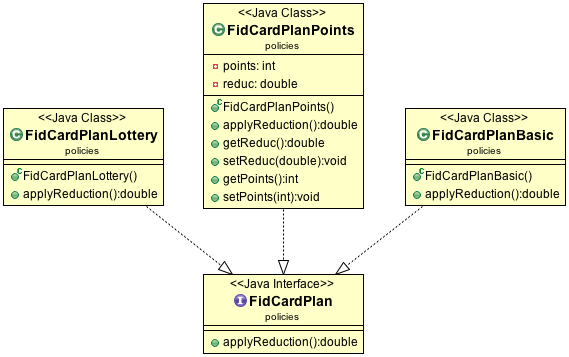
\includegraphics[scale=0.5]{./img/FidCardPlan.png}
    \end{center}
  \caption{\umld Fidelity card plan policy.}
  \label{fig:fidcardplan_uml}
\end{figure}
\begin{figure}
  \begin{center}
    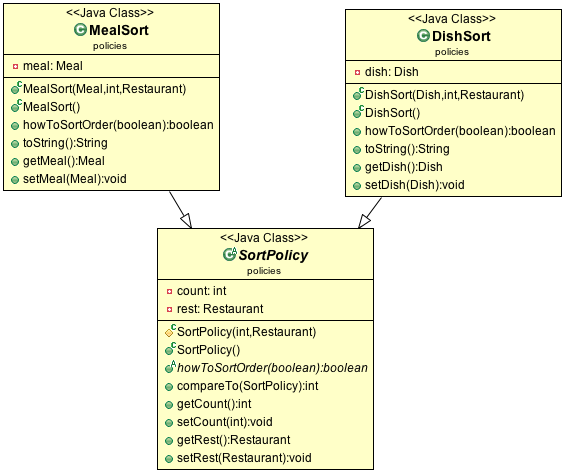
\includegraphics[scale=0.5]{./img/SortOrderPolicy.png}
    \end{center}
  \caption{\umld Sort order policy.}
  \label{fig:sortorder_uml}
\end{figure}
\begin{figure}
  \begin{center}
    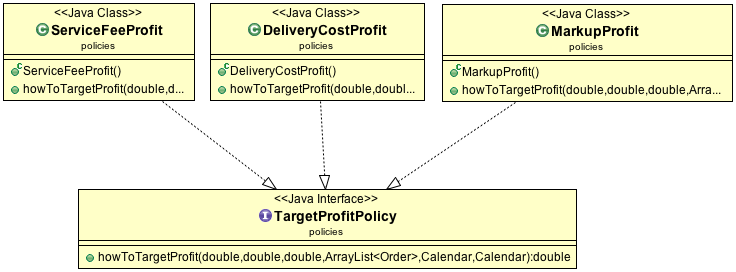
\includegraphics[scale=0.5]{./img/TargetProfitPolicy.png}
    \end{center}
  \caption{\umld Target profit policy.}
  \label{fig:targetprofit_uml}
\end{figure}
\begin{figure}
  \begin{center}
    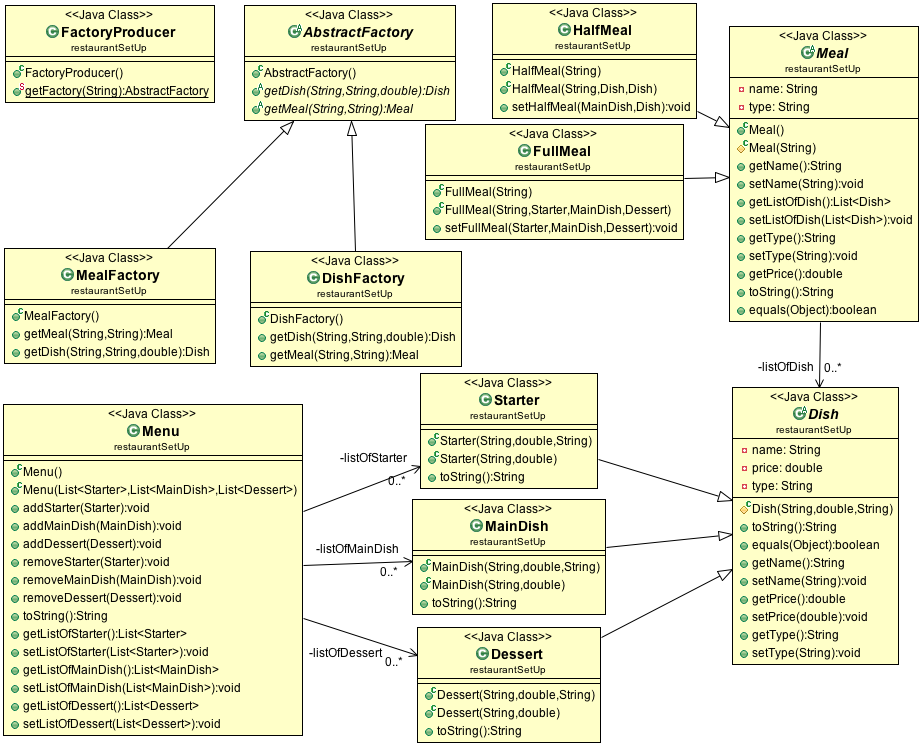
\includegraphics[scale=0.5]{./img/DishAndMeal.png}
    \end{center}
  \caption{\umld \Dish, \Meal~and related classes.}
  \label{fig:dish_meal_uml}
\end{figure}
\begin{figure}
  \begin{center}
    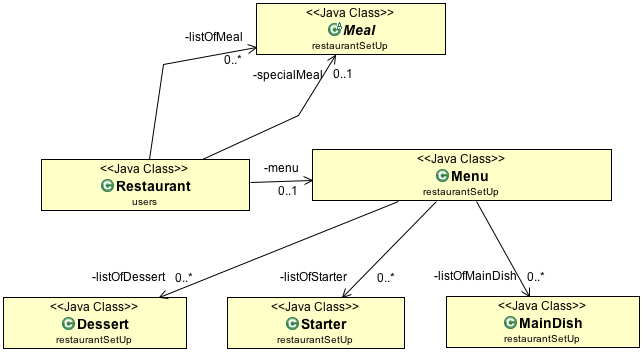
\includegraphics[scale=0.5]{./img/RestaurantToDishAndMeal.png}
    \end{center}
  \caption{\umld \Restaurant~and its links to \Dish~and \Meal.}
  \label{fig:restaurant_dish_meal_uml}
\end{figure}
\begin{figure}
  \begin{center}
    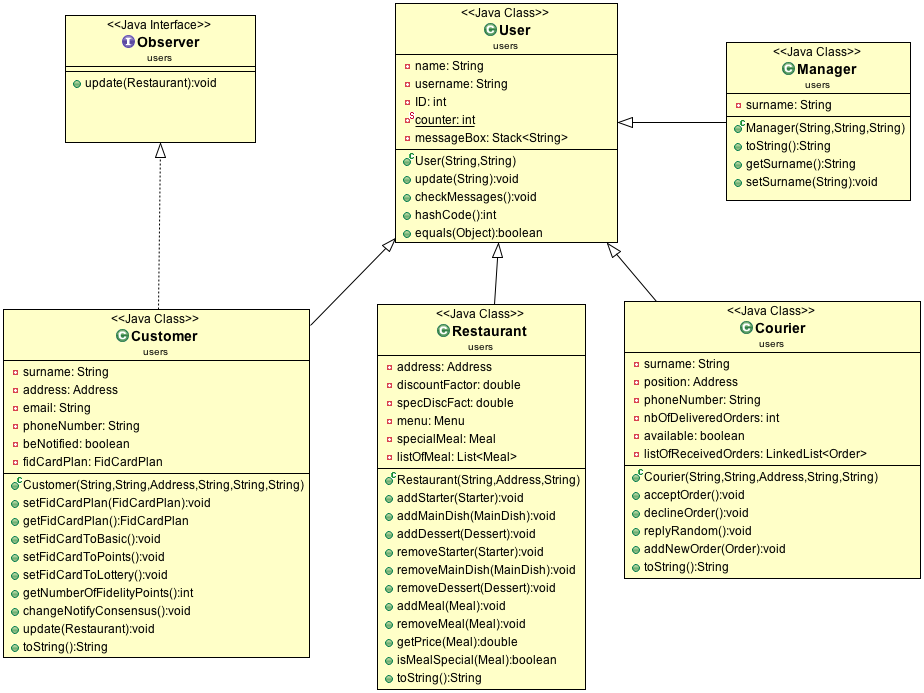
\includegraphics[scale=0.5]{./img/Users.png}
    \end{center}
  \caption{\umld \User~and its links to its subclasses.}
  \label{fig:users_uml}
\end{figure}

\begin{figure}
  \begin{center}
    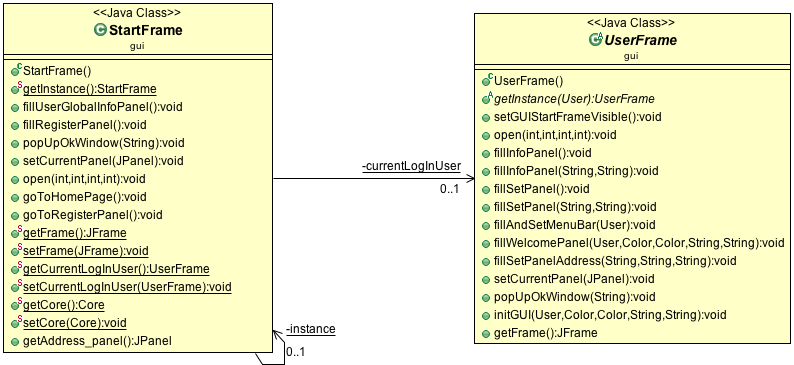
\includegraphics[scale=0.57]{./img/StartFrameToUserFrame.png}
    \end{center}
  \caption{Relationship between \StFra~and \UserF.}
  \label{fig:start2user_uml}
\end{figure}
\begin{figure}
  \begin{center}
    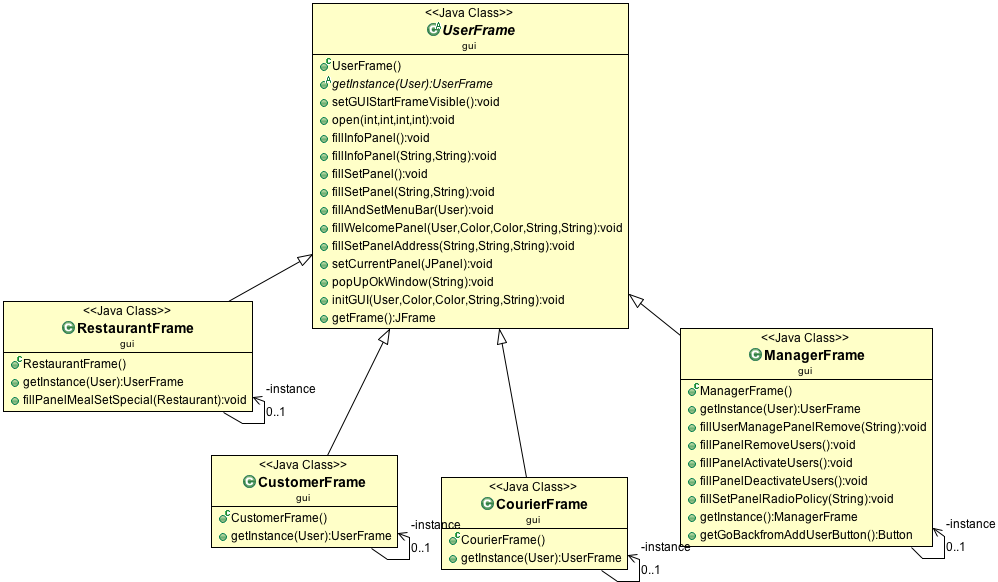
\includegraphics[scale=0.47]{./img/GUI_UserFrame_to_Users.png}
    \end{center}
  \caption{Abstact user class and users.}
  \label{fig:userframe2users_uml}
\end{figure}
\begin{figure}
  \begin{center}
    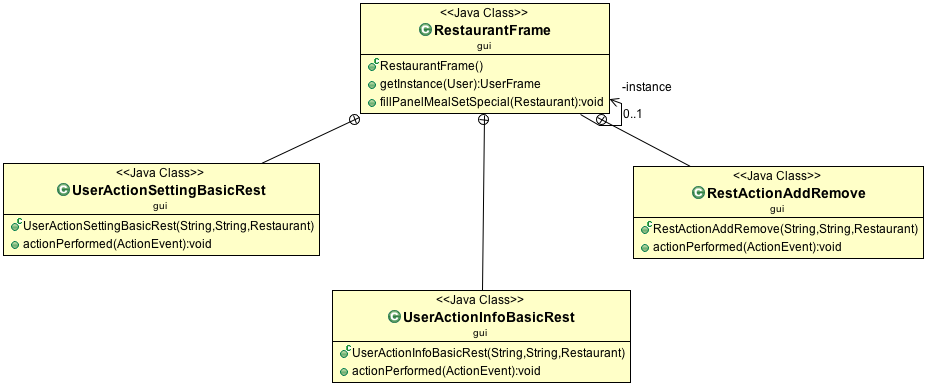
\includegraphics[scale=0.47]{./img/RestaurantFrame_NestedClasses.png}
    \end{center}
  \caption{Usage of nested classes for menu bar.}
  \label{fig:restaurantNestedClass_uml}
\end{figure}
\begin{figure}
  \begin{center}
    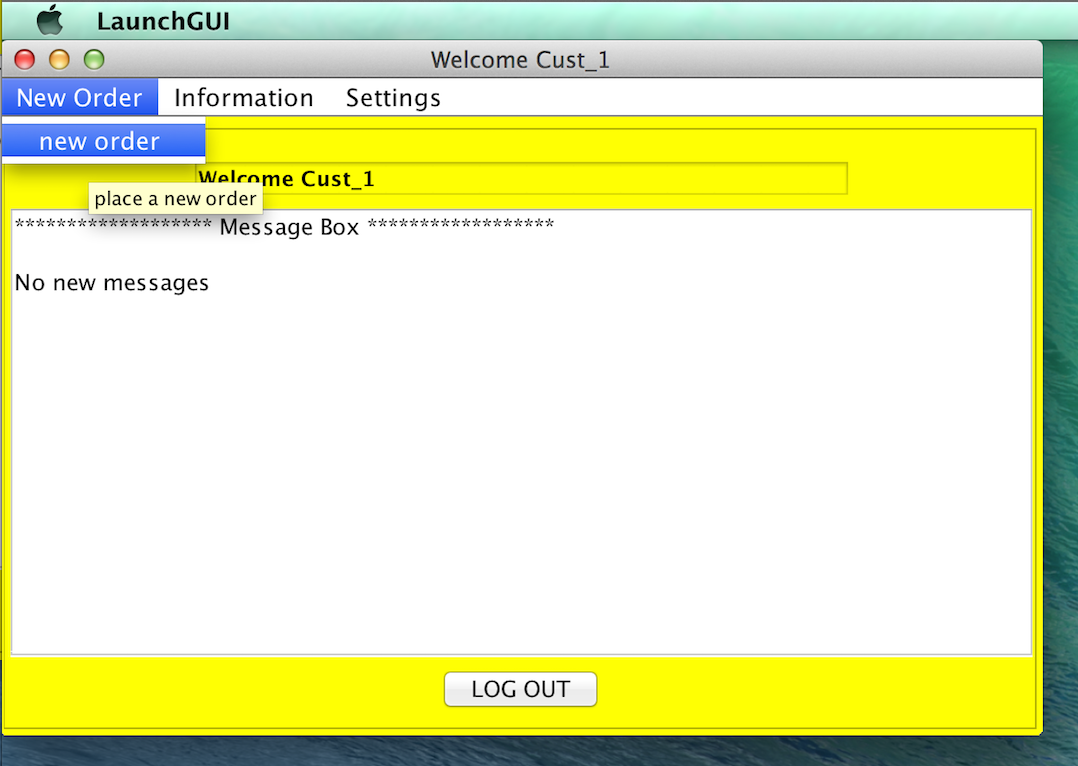
\includegraphics[scale=0.57]{./img/menuBarDescription.png}
    \end{center}
  \caption{Description of action when moving over menu item.}
  \label{fig:menuBarDescription}
\end{figure}
\begin{figure}
  \begin{center}
    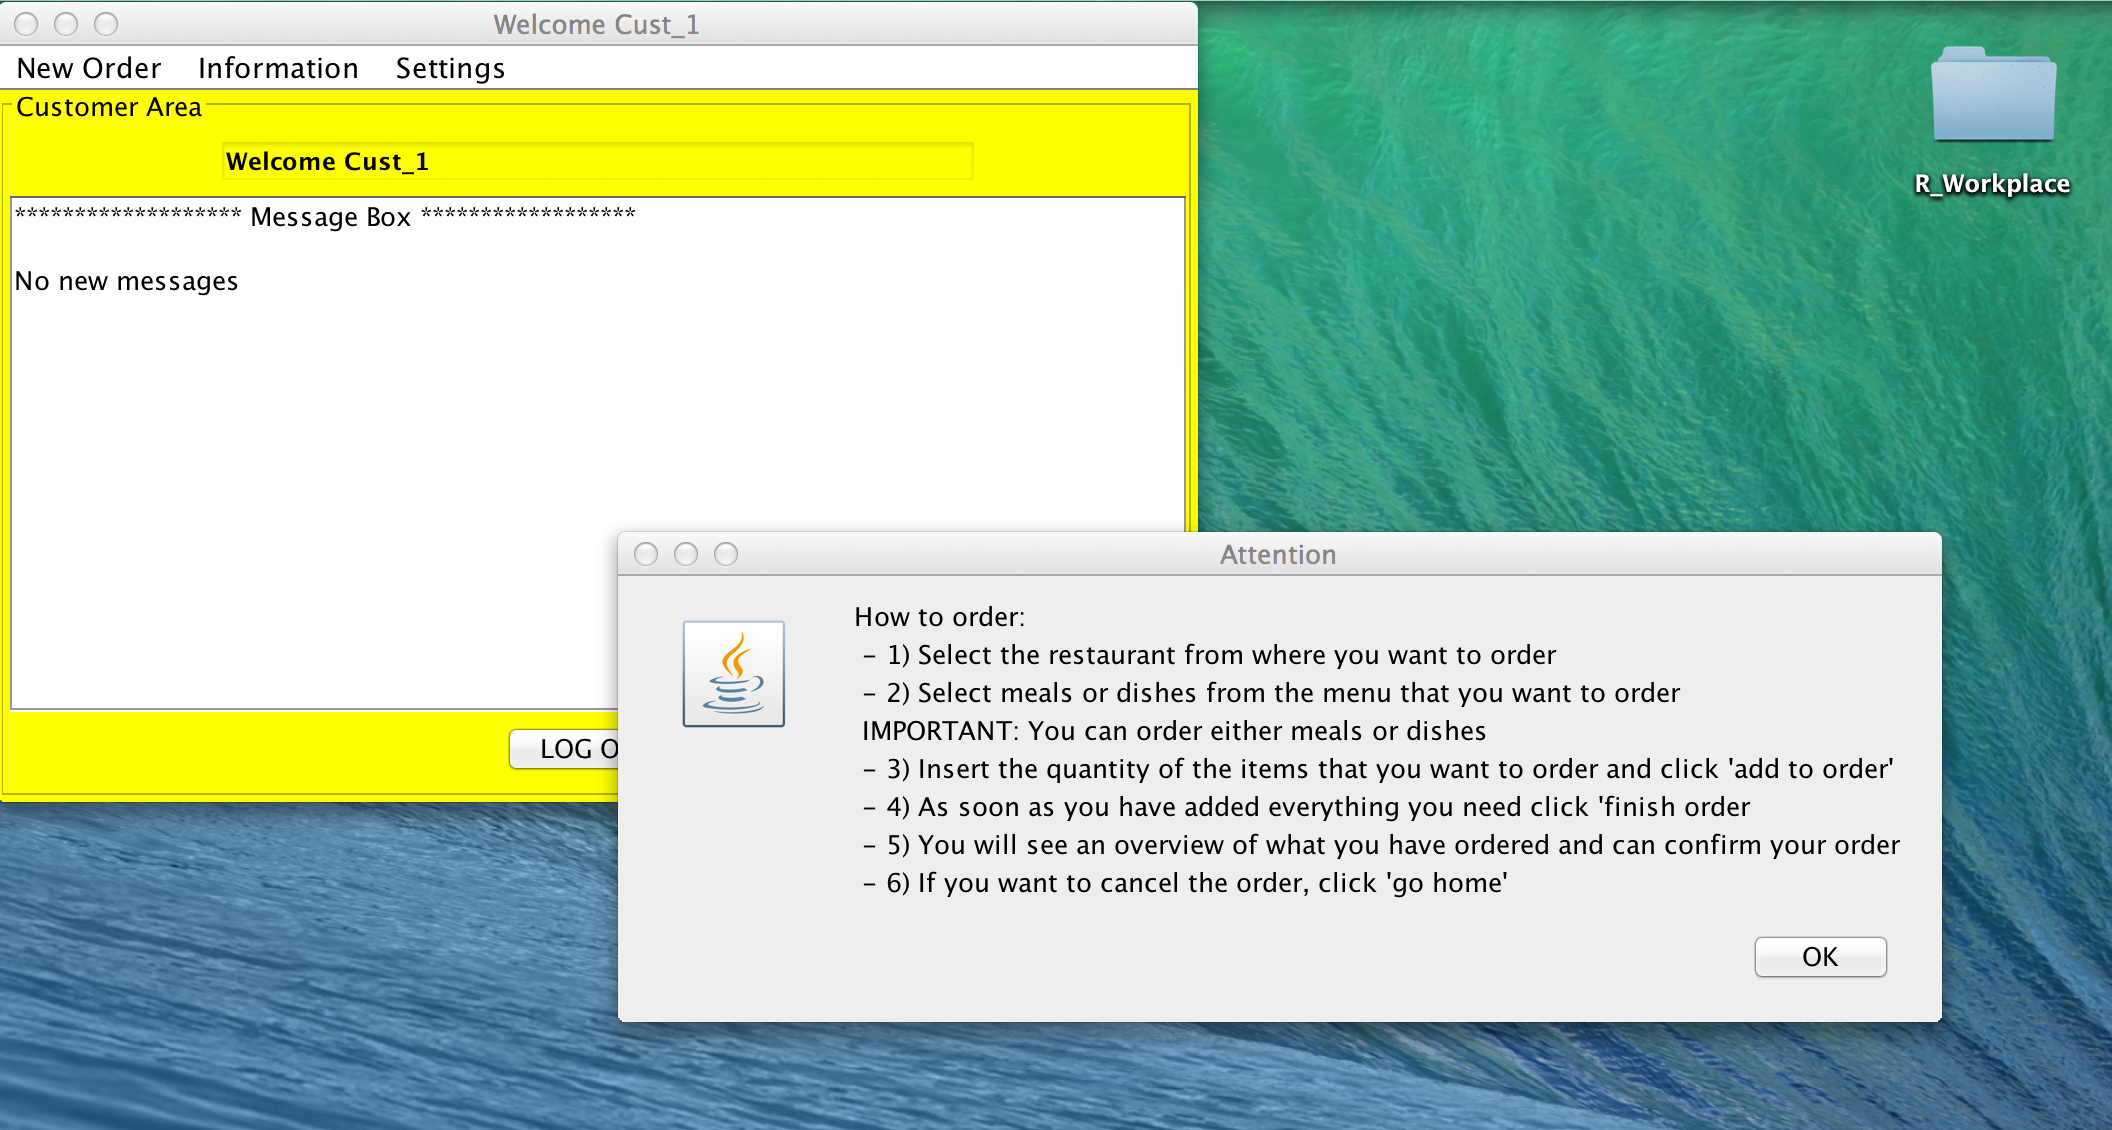
\includegraphics[scale=0.37]{./img/instructionPopUp.png}
    \end{center}
  \caption{Instuction pop up before new order function.}
  \label{fig:instructionPopUp}
\end{figure}
\begin{figure}
  \begin{center}
    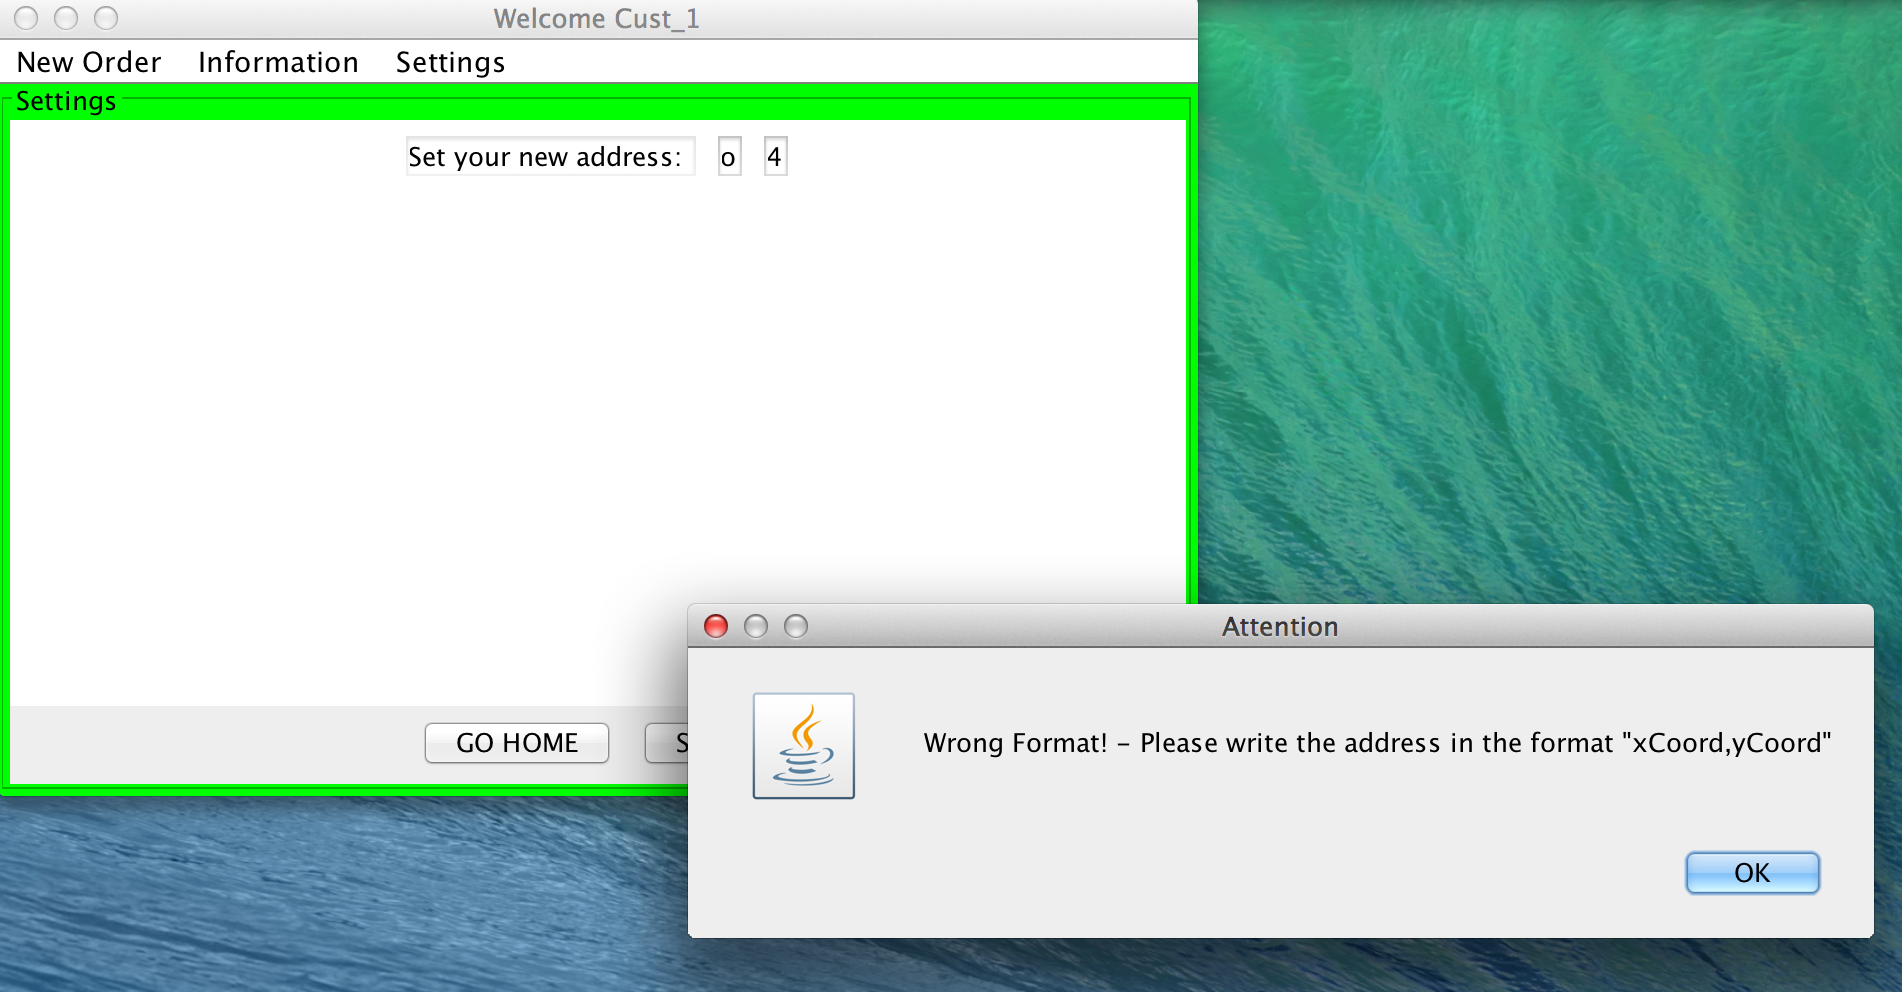
\includegraphics[scale=0.37]{./img/wrongFormat.png}
    \end{center}
  \caption{Pop up informing user of wrong entry.}
  \label{fig:wrongFormat}
\end{figure}


% section uml_class_diagrams_characteristics (end)